\documentclass{article}
\usepackage{graphicx}
\usepackage{amsmath}
\usepackage{float}
\usepackage{amsfonts}
\usepackage{listings}
\usepackage{xcolor}
\usepackage[utf8]{inputenc}
\usepackage{hyperref}
\usepackage{fancybox}
\usepackage{booktabs}
\usepackage{array}
\usepackage{tikz}
\usepackage{amsfonts}
\usepackage{dsfont}
\usepackage{pgfplots}
\pgfplotsset{compat=1.18}
\usepackage[margin=2cm]{geometry}
\usepackage[french]{babel} % Pour les éléments en français
\usetikzlibrary{shapes, arrows.meta, positioning}
\usepackage[labelfont=bf, font=small]{caption}  % Pour personnaliser le titre de la figure


\title{TP2 ADM Classification automatique}
\author{SCAIA Matteo et MARIAC Damien}
\date{\today} 

\begin{document}

\maketitle

\begin{figure}[h] 
    \centering
    
\includegraphics[width=0.5\textwidth]{ssd_logo.png} 
\end{figure}

\begin{figure}[h] 
    \centering
    
\includegraphics[width=0.5\textwidth]{logo_um_2022_rouge_RVB.png} 
\end{figure}

\newpage

\tableofcontents

\newpage
\section{Treillis de Galois}
\subsection{Introduction}
Le treillis de Galois est une structure mathématique utilisée en analyse de données pour extraire des règles d’implication. Il est construit à partir de données décrites par des propriétés booléennes, permettant de représenter les relations entre ces propriétés et les ensembles d’objets associés. 
Le treillis de Galois peut également intégrer des relations liant les données entre elles.
\subsection{Interprétation et création du treillis de Galois}
Dans cette question, nous allons analyser le treillis de Galois construit à partir des données fournies par le sujet afin de modéliser les relations entre les films et leurs caractéristiques.
\begin{figure}[h]
    \centering
    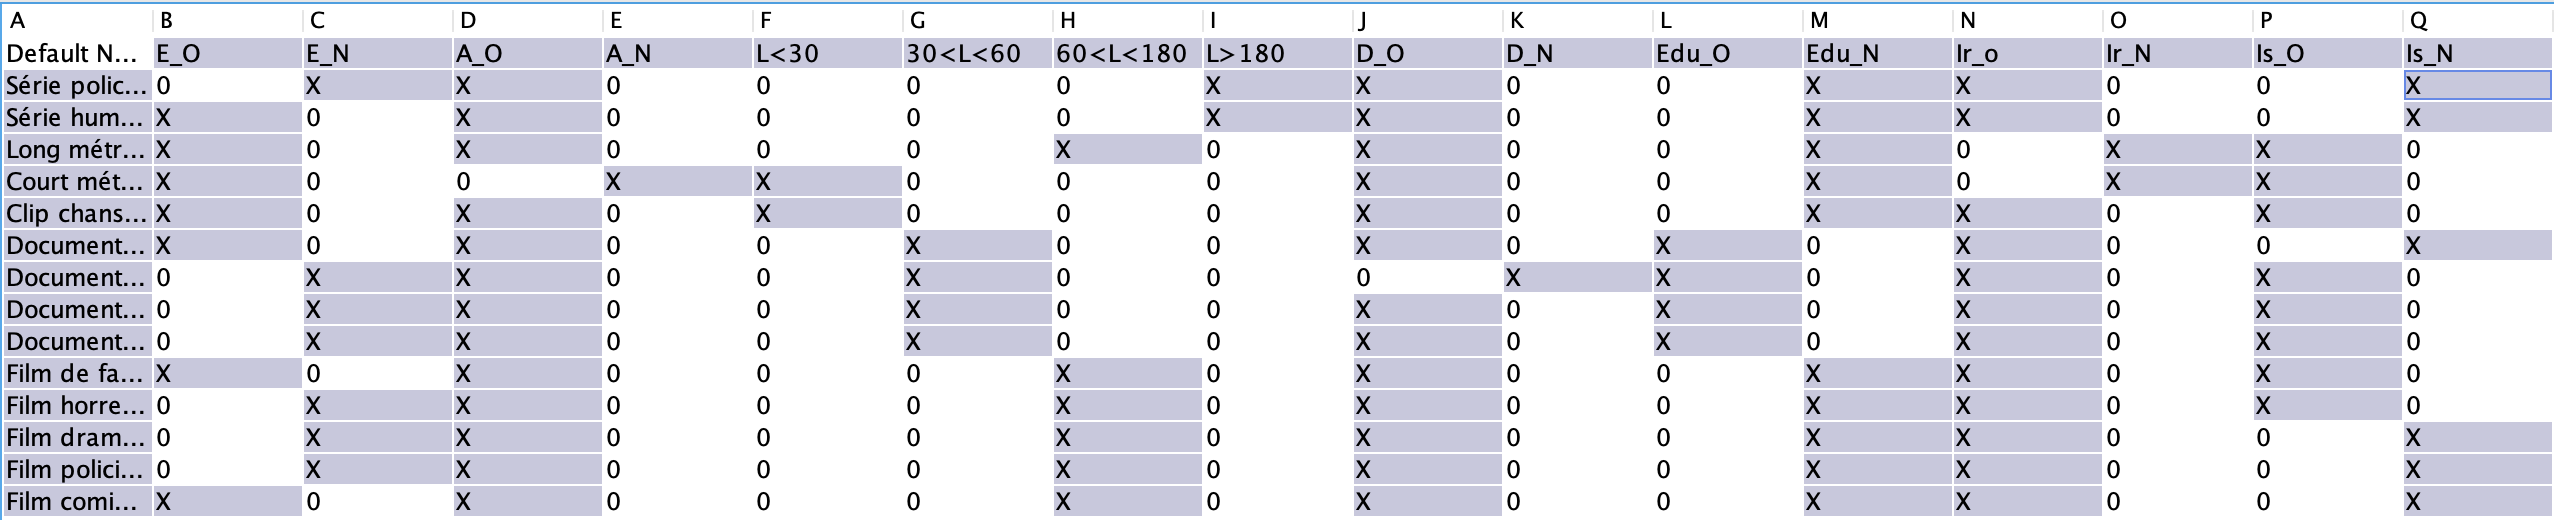
\includegraphics[width=0.7\textwidth]{tableau.png}
    \caption{Tableau des relations binaires}
    \label{fig:tableau} 
\end{figure}
\\
À l'aide du logiciel Galicia, nous obtenons le treillis de Galois suivant :
\begin{figure}[h]
    \centering
    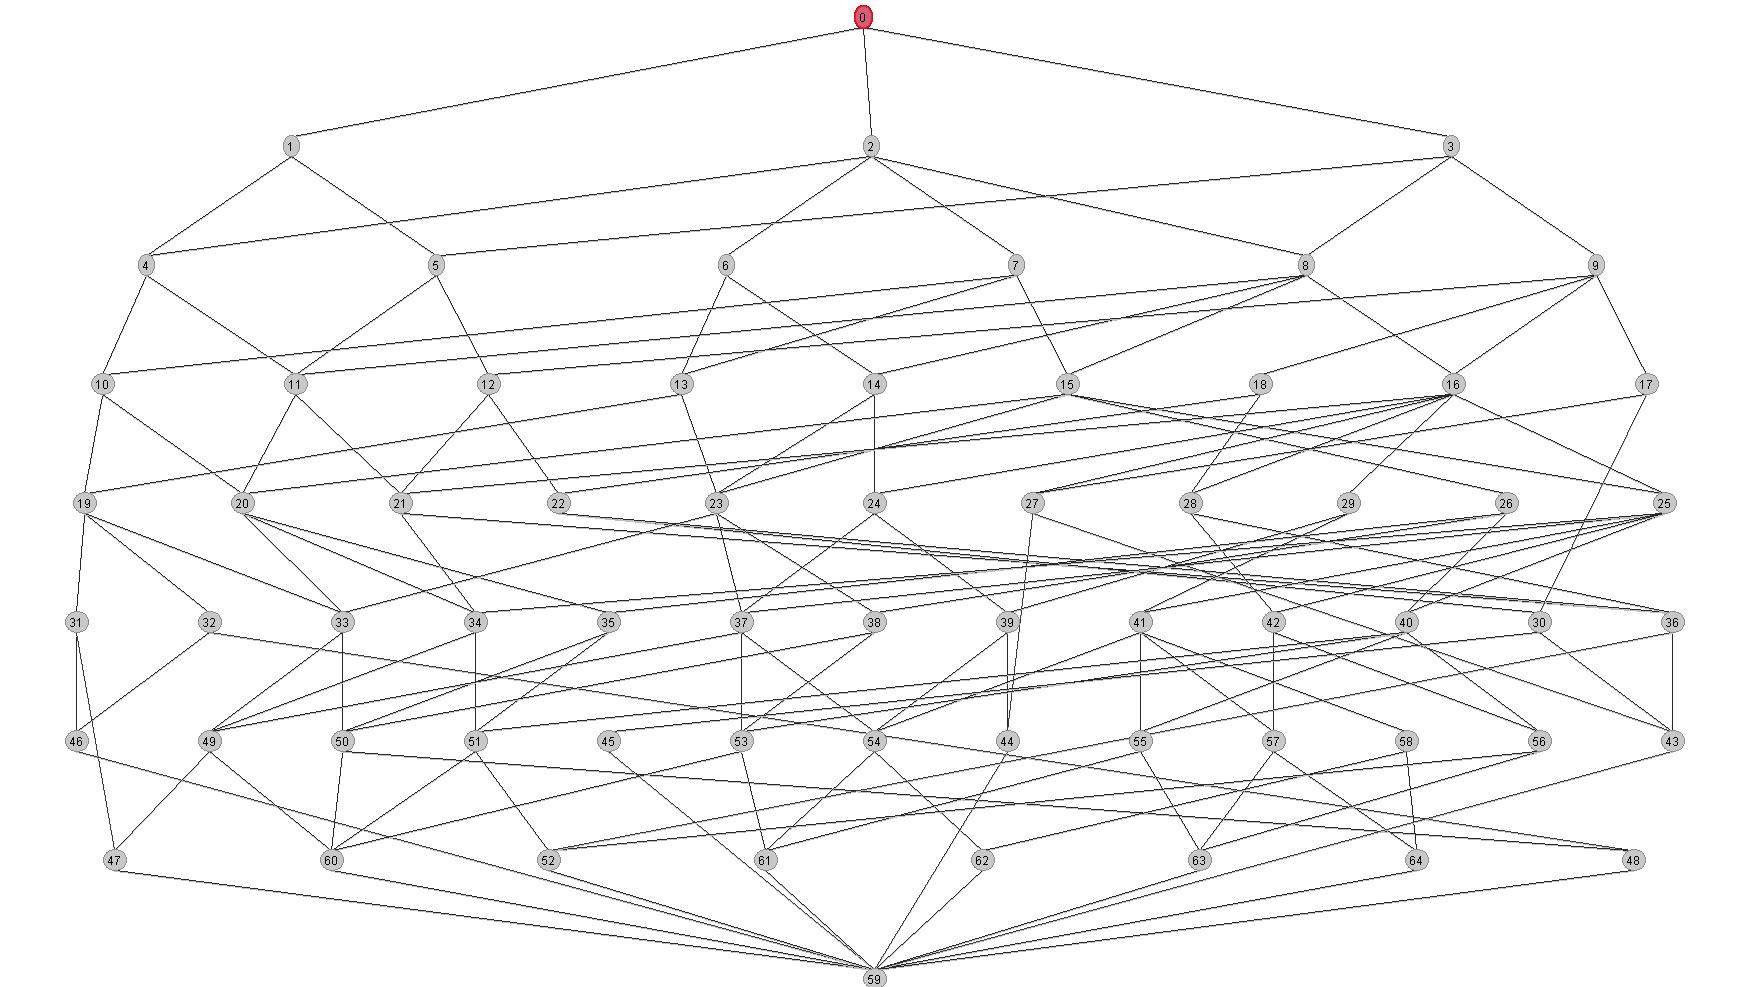
\includegraphics[width=0.7\textwidth]{treillis.png}
    \caption{Treillis de Galois de notre tableau}
    \label{fig:treillis} 
\end{figure}
\\
Dans un treillis de Galois, les nœuds situés aux extrémités correspondent soit à l’ensemble de tous les individus (en haut), soit à l’ensemble de toutes les caractéristiques (en bas). Ces nœuds étant trop généraux ou trop spécifiques, leur analyse n’est pas nécessaire.
\\
\\
Le nœud 57 regroupe les films dramatiques (FD), les films policiers (FP) et les séries policières (SP), caractérisés par les propriétés suivantes : ils s’adressent aux adolescents et aux adultes (A = Oui), ont un objectif distractif (D = Oui), ne sont pas éducatifs (ED = Non), ne ciblent pas les enfants (E = Non), utilisent des images réelles (IR = Oui) et n’incluent pas d’images de synthèse (IS = Non). Ce regroupement correspond à des œuvres qui partagent des thématiques et des intentions narratives du genre "thriller".
\\
Par ailleurs, ce nœud est lié à la classe 42, qui partage les mêmes caractéristiques mais inclut également des œuvres utilisant des images de synthèse. Cela permet d’y intégrer des films d’horreur (FH).
\\
Cette classe peut être interprétée comme un regroupement de film conçues pour provoquer du suspense ou des "frissons".
\\
\\
Le nœud 16 représente une classe large regroupant plusieurs types de films et séries partageant diverses caractéristiques : un public adulte, une vocation distractive, et des images réelles. Ce nœud est particulièrement intéressant, car il se connecte à plusieurs autres classes. Ces caractéristiques sont partagées par des genres variés. De ce fait, cette classe regroupe de nombreux types de films et séries, tels que les clips musicaux, les documentaires artistiques, les documentaires sur la nature, les documentaires scientifiques, les films comiques, les films dramatiques, les films de fantasy, les films d’horreur, ainsi que les séries humoristiques et policières.
\\
\\
On remarque également le nœud 17, qui regroupe tous les documentaires. Les caractéristiques de cette classe sont qu’elle s’adresse aux adultes (A = Oui), a une vocation éducative (ED = Oui), utilise des images réelles (IR = Oui) et correspond à des productions de courte durée (30-60 minutes). Ces caractéristiques décrivent ce que sont les documentaires.
\\



\section{Classification hiérarchique de parcelles forestières tropicales}
L4.2 -> justification a l'oral : 1 min
\subsection{Préparation des données}
\subsection{CAH des parcelles sur les densités de peuplement}
\end{document}